% vim: foldmethod=marker foldlevel=0
% -----------------------------------------------------------------------------
% Copyright &copy; 2015 Ben Blazak <bblazak@fullerton.edu>  
% This work is licensed under a [Creative Commons Attribution 4.0 International
% License] (http://creativecommons.org/licenses/by/4.0/)  
% -----------------------------------------------------------------------------

% -----------------------------------------------------------------------------
% Copyright &copy; 2015 Ben Blazak <bblazak@fullerton.edu>  
% This work is licensed under a [Creative Commons Attribution 4.0 International
% License] (http://creativecommons.org/licenses/by/4.0/)  
% -----------------------------------------------------------------------------

% - [Which lua environment should I use?] (http://tex.stackexchange.com/a/33102)
\directlua{require('scripts/functions.lua')}

\ifx\question\undefined
  \long\def \question #1{#1}
\fi
\ifx\answer\undefined
  \long\def \answer #1{#1}
\fi

% -----------------------------------------------------------------------------

\def \docTitle  {\directlua{tex.print(doc_title('\jobname'))}}
\def \docAuthor {\question{Name:\hfill{}CWID:\hfill}\answer{Answer Key}}
\def \docClass  {CPSC 121-11}
\def \docSchool {~}
\def \docTerm   {CSUF Fall 2015}

\def \docCopyright {
  \begin{figure}[b!]
    \tiny
    {\answer{\color{red}}\question{\color{.}}\hrule}
    \vspace{2ex}
    \begin{minipage}[c]{0.10\textwidth} \vspace{0ex} \vspace{-1pt}
      
\includegraphics[height=5ex]{images/ccby}
    \end{minipage}
    \begin{minipage}[c]{0.90\textwidth} \vspace{0ex}
      Copyright \copyright{} Ben Blazak \url{bblazak@fullerton.edu}\\
      This work is licensed under a Creative Commons Attribution 4.0
      International License \url{http://creativecommons.org/licenses/by/4.0/}
    \end{minipage}
    \vspace{-.14in}
    \vspace{2ex}
  \end{figure}
}

% -----------------------------------------------------------------------------

\documentclass{article}

\usepackage[includehead,
%             includefoot,
            margin=1in,
            top=.25in,
            headheight=.75in,
            headsep=.25in,
            footskip=.25in,
           ]{geometry}

\usepackage[export]{adjustbox}
\usepackage[fleqn]{amsmath}
\usepackage{amssymb}
\usepackage[shortlabels]{enumitem}
\usepackage{etoolbox}
\usepackage{fancyhdr}
\usepackage{lastpage}
\usepackage[cachedir={.minted-\jobname}]{minted}
\usepackage{tcolorbox}
\usepackage{tikz}
\usepackage[explicit]{titlesec}

\usepackage[T1]{fontenc}
\usepackage[utf8]{inputenc}
\usepackage{lmodern}

\usepackage{xcolor}

% - [Illegal parameter number in definition of \Hy@tempa]
%   (https://kba49.wordpress.com/2013/04/12/illegal-parameter-number-in-definition-of-hytempa/)
\usepackage{hyperref}

% text ------------------------------------------------------------------------

\binoppenalty = 10000  % never break next to a binary operator
\relpenalty   = 10000  % never break next to a relation operator

\setlength{\parindent}{0em}
\setlength{\parskip}{1ex}

\setlist[itemize]{nosep,itemsep=.5ex,parsep=.5ex}

% sections --------------------------------------------------------------------

% - <http://tex.stackexchange.com/a/58299>
\titleformat{name=\section}[block]{\normalfont\Large\bfseries}{}{0em}{#1\ \thesection}
% - <http://tex.stackexchange.com/a/102120>
\titleformat{name=\section,numberless}[block]{\normalfont\Large\bfseries}{}{0em}{#1}

% math ------------------------------------------------------------------------

\setlength{\mathindent}{1cm}

% - "\begin{document}" resets these values, so they have to be treated
%   specially
\AtBeginDocument{
  \setlength{\abovedisplayskip}{1.5ex plus .5ex minus .5ex}
  \setlength{\belowdisplayskip}{1.5ex plus .5ex minus .5ex}
}

% source code -----------------------------------------------------------------

\usemintedstyle{solarizedlight}
\setminted{frame=single}

\fvset{samepage=true}

% header and footer -----------------------------------------------------------

\pagestyle{fancy}

\renewcommand{\headrule}{{\answer{\color{red}}\question{\color{.}}
                          \vskip 0.5ex \hrule height 0.4pt \vskip 0.5ex}}
\renewcommand{\footrule}{{\answer{\color{red}}\question{\color{.}}
                          \vskip 0.5ex \hrule height 0.4pt \vskip 0.5ex}}

\fancyhead[L]{{\answer{\color{red}}\question{\color{.}}\docAuthor}
              {\color{.}\\\docClass}}
\fancyhead[C]{{\color{.}\docSchool\\}}
\fancyhead[R]{{\color{.}\docTerm\\\docTitle}}

\fancyfoot[C]{\thepage{} of \pageref{LastPage}}

% -----------------------------------------------------------------------------
% macros
% -----------------------------------------------------------------------------

% abbreviations ---------------------------------------------------------------

\def \<{\langle}
\def \>{\rangle}

\def \ε{\varepisilon}
\def \θ{\vartheta}
\def \κ{\varkappa}
\def \π{\varpi}
\def \ρ{\varrho}
\def \σ{\varsigma}
\def \φ{\varphi}

\def \Γ{\varGamma}
\def \Δ{\varDelta}
\def \Θ{\varTheta}
\def \Λ{\varLambda}
\def \Ξ{\varXi}
\def \Π{\varPi}
\def \Σ{\varSigma}
\def \Υ{\varUpsilon}
\def \Φ{\varPhi}
\def \Ψ{\varPsi}
\def \Ω{\varOmega}

% special characters ----------------------------------------------------------

\catcode `α = \active \let α \alpha
\catcode `β = \active \let β \beta
\catcode `γ = \active \let γ \gamma
\catcode `δ = \active \let δ \delta
\catcode `ε = \active \let ε \epsilon
\catcode `ζ = \active \let ζ \zeta
\catcode `η = \active \let η \eta
\catcode `θ = \active \let θ \theta
\catcode `ι = \active \let ι \iota
\catcode `κ = \active \let κ \kappa
\catcode `λ = \active \let λ \lambda
\catcode `μ = \active \let μ \mu
\catcode `ν = \active \let ν \nu
\catcode `ξ = \active \let ξ \xi
\catcode `ο = \active \let ο o
\catcode `π = \active \let π \pi
\catcode `ρ = \active \let ρ \rho
\catcode `σ = \active \let σ \sigma
\catcode `τ = \active \let τ \tau
\catcode `υ = \active \let υ \upsilon
\catcode `φ = \active \let φ \phi
\catcode `χ = \active \let χ \chi
\catcode `ψ = \active \let ψ \psi
\catcode `ω = \active \let ω \omega

\catcode `Α = \active \let Α A
\catcode `Β = \active \let Β B
\catcode `Γ = \active \let Γ \Gamma
\catcode `Δ = \active \let Δ \Delta
\catcode `Ε = \active \let Ε E
\catcode `Ζ = \active \let Ζ Z
\catcode `Η = \active \let Η H
\catcode `Θ = \active \let Θ \Theta
\catcode `Ι = \active \let Ι I
\catcode `Κ = \active \let Κ K
\catcode `Λ = \active \let Λ \Lambda
\catcode `Μ = \active \let Μ M
\catcode `Ν = \active \let Ν N
\catcode `Ξ = \active \let Ξ \Xi
\catcode `Ο = \active \let Ο O
\catcode `Π = \active \let Π \Pi
\catcode `Ρ = \active \let Ρ P
\catcode `Σ = \active \let Σ \Sigma
\catcode `Τ = \active \let Τ T
\catcode `Υ = \active \let Υ \Upsilon
\catcode `Φ = \active \let Φ \Phi
\catcode `Χ = \active \let Χ X
\catcode `Ψ = \active \let Ψ \Psi
\catcode `Ω = \active \let Ω \Omega

% other -----------------------------------------------------------------------

\def \docCodeDir {./code/\directlua{tex.print(jobname_root('\jobname'))}/}
\def \docImageDir {./images/\directlua{tex.print(jobname_root('\jobname'))}/}

\long\def \textAnswer #1{\answer{{\color{red!50!black}#1}}}
\long\def \textQuestion #1{\question{{\color{.}#1}}}

\long\def \standardsSection #1{{
  \section*{Standards}
  \def\arraystretch{2}
  \setlength\tabcolsep{1em}
  \begin{tabular}{|r|l|}
    \hline \textbf{Standard} & \textbf{Score} \\\hline #1
  \end{tabular}
  \docCopyright
  \newpage
}
  \def\docCopyright{}
}
\long\def \standards #1{{
  \vspace{-1em}
  \def\arraystretch{2}
  \setlength\tabcolsep{1em}
  \begin{tabular}{|r|l|}
    \hline #1
  \end{tabular}
  \vspace{1em}
}}
\def \standard #1{
  #1 & ~~~ \\\hline
}

\def \evaluateCodeTop #1#2{
  \def\codeFile{\docCodeDir/.#1.cpp.gen.section.#2}
  \IfFileExists{\docCodeDir/.#1.gen.output.gen.section.#2}
               {\def\outputFile{\docCodeDir/.#1.gen.output.gen.section.#2}}
               {\def\outputFile{\docCodeDir/.#1.gen.output.gen.section.all}}
  \par
  \inputminted{cpp}{\codeFile}
  \textQuestion{
    \inputminted[label={\normalsize{}Output},fontsize=\Large]{text}
      {\outputFile.gen.blank}
  }
  \textAnswer{
    \inputminted[label={\normalsize{}Output},fontsize=\Large]{text}
      {\outputFile}
  }
  \par
}
\def \evaluateCodeLeft #1#2{
  \def\codeFile{\docCodeDir/.#1.cpp.gen.section.#2}
  \IfFileExists{\docCodeDir/.#1.gen.output.gen.section.#2}
               {\def\outputFile{\docCodeDir/.#1.gen.output.gen.section.#2}}
               {\def\outputFile{\docCodeDir/.#1.gen.output.gen.section.all}}
  \par
  \begin{minipage}[t]{0.5\linewidth} \vspace{0ex}
    \inputminted{cpp}{\codeFile}
  \end{minipage}
  \begin{minipage}[t]{0.5\linewidth} \vspace{0ex}
    \textQuestion{
      \inputminted[label=Output]{text}{\codeFile.gen.blank}
    }
    \textAnswer{
      \inputminted[label=Output]{text}{\outputFile}
    }
  \end{minipage}
  \par
}

\def \showCodeTop #1#2{
  \def\codeFile{\docCodeDir/.#1.cpp.gen.section.#2}
  \IfFileExists{\docCodeDir/.#1.gen.output.gen.section.#2}
               {\def\outputFile{\docCodeDir/.#1.gen.output.gen.section.#2}}
               {\def\outputFile{\docCodeDir/.#1.gen.output.gen.section.all}}
  \par
  \inputminted{cpp}{\codeFile}
  \vspace{0.5\parskip}
  \inputminted[label=Output]{text}{\outputFile}
  \par
}
\def \showCodeLeft #1#2{
  \def\codeFile{\docCodeDir/.#1.cpp.gen.section.#2}
  \IfFileExists{\docCodeDir/.#1.gen.output.gen.section.#2}
               {\def\outputFile{\docCodeDir/.#1.gen.output.gen.section.#2}}
               {\def\outputFile{\docCodeDir/.#1.gen.output.gen.section.all}}
  \par
  \begin{minipage}[t]{0.5\linewidth} \vspace{0ex}
    \inputminted{cpp}{\codeFile}
  \end{minipage}
  \begin{minipage}[t]{0.5\linewidth} \vspace{0ex}
    \inputminted[label=Output]{text}{\outputFile}
  \end{minipage}
  \par
}



\def \memoryImage{%
  \par\medskip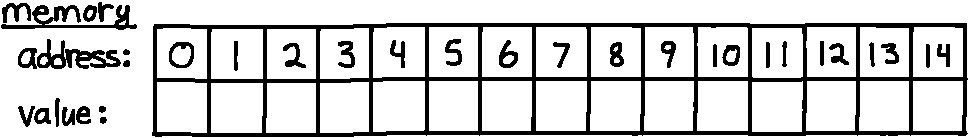
\includegraphics[width=\linewidth,valign=t]{\docImageDir/memory}%
}

% -----------------------------------------------------------------------------

\begin{document}
\docCopyright

% -----------------------------------------------------------------------------

\standardsSection{
  \hline\hline
  \standard{documentation}
  \standard{consistency of style}
  \hline\hline
  \standard{debugging and testing correctness}
  \standard{type declarations}
  \standard{pointers and references}
  \standard{memory management and dynamic memory}
  \hline\hline
  \standard{classes}
  \standard{inheritance}
  \standard{interfaces}
  \hline\hline
  \standard{data types and representation}
  \standard{operators}
  \standard{control flow}
  \standard{arrays}
  \standard{functions}
  \standard{file I/O}
  \hline\hline
  \standard{review :: general knowledge}
  \standard{object-oriented programming :: general knowledge}
}

% -----------------------------------------------------------------------------
%   \standard{debugging and testing correctness}
% {{{

\newpage

\section{Question}
\standards{
  \standard{debugging and testing correctness}
}

\vspace{1.5ex}
\begin{itemize}

    \filbreak
  \item Correct this code so that it produces the intended output.
    \correctCodeTop{debugging}{if}
    \vspace{3ex}

    \filbreak
  \item Correct this code so that it produces the intended output.
    \correctCodeTop{debugging}{while}
    \vspace{3ex}

    \filbreak
  \item Correct this code so that it produces the intended output.
    \correctCodeTop{debugging}{do-while}
    \vspace{3ex}

    \filbreak
  \item Correct the code below so that it produces the intended output, and
    answer the following question:
    \begin{itemize}
      \item How many times does this loop, as originally written, run? (circle
        one)
        \begin{itemize}
          \item 0 times
          \item 1 time
          \item many times
          \item infinitely
        \end{itemize}
    \end{itemize}
    \correctCodeTop{debugging}{for}
    \vspace{3ex}
    \newpage

    \filbreak
  \item Correct the portion of this code that probably doesn't do what the
    writer intended.
    \correctCodeTop{debugging}{or}
    \vspace{3ex}

\end{itemize}

% }}}
% -----------------------------------------------------------------------------
%   \standard{type declarations}
% {{{

\newpage

\section{Question}
\standards{
  \standard{type declarations}
}

\section*{Instructions}

{
  \long\def\answer#1{#1}
  Write declarations for the following descriptions, and descriptions for the
  following declarations:
  \begin{itemize}
    \item \mintinline{cpp}{int i}
      \textAnswer{\par{}declare i as int}
    \item declare a as array 3 of int
      \textAnswer{\par{}\mintinline{cpp}{int a[3]}}
  \end{itemize}
}

\section*{Questions}

Write declarations for the following descriptions, and descriptions for the
following declarations:
\begin{itemize}

  \item \mintinline{cpp}{int i}
    \textAnswer{\par{}declare i as int}
    \vfill

  \item declare a as array 3 of int
    \textAnswer{\par{}\mintinline{cpp}{int a[3]}}
    \vfill

  \item \mintinline{cpp}{int (*p)[3]}
    \textAnswer{\par{}declare p as pointer to array 3 of int}
    \vfill

  \item declare p as pointer to int
    \textAnswer{\par{}\mintinline{cpp}{int * p}}
    \vfill

  \item \mintinline{cpp}{int & r}
    \textAnswer{\par{}declare r as reference to int}
    \vfill

  \item declare r as reference to array 3 of int
    \textAnswer{\par{}\mintinline{cpp}{int (&r)[3]}}
    \vfill

  \item \mintinline{cpp}{void (*p)()}
    \textAnswer{\par{}declare p as pointer to function returning void}
    \vfill

  \item declare p as pointer to function (int, array of int) returning int
    \textAnswer{\par{}\mintinline{cpp}{int (*p)(int, int[])}}
    \vfill

\end{itemize}

% }}}
% -----------------------------------------------------------------------------
%   \standard{pointers and references}
% {{{

\newpage

\section{Question}
\standards{
  \standard{pointers and references}
}

\begin{itemize}

  \item Write statements to do the following:
    \begin{itemize}
      \item Declare a float, and set it equal to 3.14.
      \item Declare a pointer to the float, and use it to increment the float
        by 2.
      \item Declare a reference to the float, and use it to set the float
        equal to 7.25.
      \item Output the final value of the float using 1) the float, 2) the
        pointer to the float, and 3) the reference to the float, separated by
        whitespace.
    \end{itemize}
    \textAnswer{\showCodeLeft{pointers-1}{all}}
    \vfill

  \item Show the output of the following program:
    \evaluateCodeLeft{pointers-2}{all}

    \filbreak

  \item Show the output of the following program.  Recall that
    \mintinline{cpp}{uintptr_t} is an unsigned integer type capable of
    storing any valid pointer value without loss of precision, and that
    \mintinline{cpp}{(uintptr_t)a} is a C style cast of \mintinline{cpp}{a} to
    type \mintinline{cpp}{uintptr_t}.
    \evaluateCodeTop{pointers-3}{all}
    \vspace{3ex}

  \item List one similarity between an array and a pointer to the array's first
    element.
    \textAnswer{\par
      \begin{itemize}
        \item Either may be used to access any element of the array, with the
          same syntax.
        \item They both convert to the same integral value.
        \item $\cdots$
      \end{itemize}
    }
    \vfill

  \item List one difference between an array and a pointer to the array's first
    element.
    \textAnswer{\par
      \begin{itemize}
        \item They have different type.
        \item The pointer may be assigned to, whereas the array may not.
        \item Taking \mintinline{cpp}{sizeof(p)} and
          \mintinline{cpp}{sizeof(a)} (assuming the array is called
          \mintinline{cpp}{a} and the pointer is called \mintinline{cpp}{p})
          will give different results.
        \item $\cdots$
      \end{itemize}
    }
    \vfill

\end{itemize}

% }}}
% -----------------------------------------------------------------------------
%   \standard{memory management and dynamic memory}
% {{{

\newpage

\section{Question}
\standards{
  \standard{memory management and dynamic memory}
}

\begin{itemize}

  \item Using either the C style functions or the C++ style operators, write
    statements to do the following:
    \begin{itemize}
      \item Dynamically allocate memory for an array of 5
        \mintinline{cpp}{int}s, and store the resulting pointer to the first
        element in a variable of the appropriate type.
      \item Deallocate the dynamically allocated memory.
    \end{itemize}
    \textAnswer{\inputminted{cpp}{\docCodeDir/.memory.cpp.gen.section.all}}
    \vfill

  \item In what section of memory are automatic variables placed?
    \textAnswer{\par
      the stack
    }
    \vfill

  \item In what section of memory are dynamically allocated variables placed?
    \textAnswer{\par
      the heap (when using C style functions) or the free store (when using C++
      style operators) (though the free store is often informally referred to
      as the heap)
    }
    \vfill

  \item What happens when you dynamically allocate memory, but fail to
    deallocate it?
    \textAnswer{\par
      The memory remains allocated to your program until the program is
      terminated (at which time \textit{all} memory in use by your program is
      reclaimed by the operating system).  This is known as a memory leak.
    }
    \vfill

  \item What happens when you deallocate a block of dynamically allocated
    memory, but keep a pointer to the beginning of the block?
    \textAnswer{\par
      The pointer may still be used in some ways, but dereferencing it leads to
      undefined behavior.  This is known as a dangling pointer.
    }
    \vfill

\end{itemize}

% }}}
% -----------------------------------------------------------------------------
%   \standard{documentation}
%   \standard{consistency of style}
%   \standard{classes}
%   \standard{inheritance}
% {{{

\newEvenPage

\section{Question}
\standards{
  \standard{documentation}
  \standard{consistency of style}
  \standard{classes}
  \standard{inheritance}
}

% mostly from reassessment-07

Preface your program with a block comment containing a short description of
what it does, and with all necessary \mintinline{cpp}{#include} directives and
\mintinline{cpp}{using} statements.

Next, write a \mintinline{cpp}{Character} class with the following members:
\begin{itemize}
  \item A \mintinline{cpp}{name}, as a string, with either
    \mintinline{cpp}{private} or \mintinline{cpp}{protected} visibility.
  \item A default constructor that optionally accepts a constant reference to a
    \mintinline{cpp}{string} and initializes the \mintinline{cpp}{name} data
    member to that value.
  \item A \mintinline{cpp}{void} method named \mintinline{cpp}{sayName} that
    prints \mintinline{cpp}{"My name is "} followed by the
    \mintinline{cpp}{Character}'s name, followed by a newline, to standard
    output.
\end{itemize}

Next, write an \mintinline{cpp}{AvatarCharacter} class that inherits from
\mintinline{cpp}{Character} and has the following members:
\begin{itemize}
  \item An \mintinline{cpp}{element}, as a string, with either
    \mintinline{cpp}{private} or \mintinline{cpp}{protected} visibility.
  \item A default constructor that optionally accepts two constant references
    to \mintinline{cpp}{string}s, passes the first value to the parent
    constructor, and uses the second to initialize the
    \mintinline{cpp}{element} data member.
  \item A \mintinline{cpp}{void} function named \mintinline{cpp}{sayElement}
    that sends \mintinline{cpp}{"I bend "}, followed by the
    \mintinline{cpp}{AvatarCharacter}'s \mintinline{cpp}{element}, followed by
    a newline, to standard output.
\end{itemize}

Finally, write a short \mintinline{cpp}{main()} that calls the
\mintinline{cpp}{sayName()} and \mintinline{cpp}{sayElement()} methods on
objects of type \mintinline{cpp}{AvatarCharacter} to produce the following
output:
\inputminted[label=Output]{text}{\docCodeDir/.classes.gen.output}

Before you begin, please
\begin{itemize}
  \item Be sure to write your answers neatly and in a good and consistent
    style.  This will be graded.  I recommend writing out your solution on
    scratch paper, and then copying it to the following page.  You might also
    consider using pencil, if pen is your usual choice.
  \item Try to comment with the level of detail you would find helpful (but not
    irritating) in code of similar complexity written by another student in
    this class.
\end{itemize}

\newpage

\textQuestion{\makePageQuadrilleRuled}
\textAnswer{\inputminted{cpp}{\docCodeDir/.classes.cpp.gen.section.all}}

\newOddPage

\textQuestion{\makePageQuadrilleRuled}
\textAnswer{~}

% }}}
% -----------------------------------------------------------------------------
%   \standard{documentation}
%   \standard{consistency of style}
%   \standard{interfaces}
% {{{

\newEvenPage

\section{Question}
\standards{
  \standard{documentation}
  \standard{consistency of style}
  \standard{interfaces}
}

Recall that an interface is an abstract class, and an abstract class is a class
with at least one pure \mintinline{cpp}{virtual} method.

Before you begin, please
\begin{itemize}
  \item Be sure to place at the top of your answer any necessary
    \mintinline{cpp}{#include} directives or \mintinline{cpp}{using}
    statements.
  \item Remember to preface your interface with a block comment containing a
    short description of what it is intended to represent or be used for, etc.
  \item Remember to include a \mintinline{cpp}{virtual} destructor with a
    default inline implementation.  \textbf{All interfaces classes should have
    a \mintinline{cpp}{virtual} destructor.}
  \item Be sure to write your answers neatly and in a good and consistent
    style.  This will be graded.  I recommend writing out your solution on
    scratch paper, and then copying it to the following page.  You might also
    consider using pencil, if pen is your usual choice.
  \item Try to comment with the level of detail you would find helpful (but not
    irritating) in code of similar complexity written by another student in
    this class.
\end{itemize}

Write an interface for a \mintinline{cpp}{Person} having the following
\mintinline{cpp}{private} data members (all of type \mintinline{cpp}{int}):

\begin{itemize}
  \item \mintinline{cpp}{body}
  \item \mintinline{cpp}{soul}
  \item \mintinline{cpp}{mind}
  \item \mintinline{cpp}{magic}
\end{itemize}

Write \mintinline{cpp}{virtual} getters and setters, with inline
implementations, for at least two of the private data members.

Write declarations for at least two of the following pure
\mintinline{cpp}{virtual} methods (all of which take no arguments and return
\mintinline{cpp}{void}):
\begin{itemize}
  \item \mintinline{cpp}{attack}
  \item \mintinline{cpp}{defend}
  \item \mintinline{cpp}{heal}
  \item \mintinline{cpp}{cast}
\end{itemize}

\newpage

\textQuestion{\makePageQuadrilleRuled}
\textAnswer{\inputminted{cpp}{\docCodeDir/.interfaces.cpp.gen.section.all}}

% }}}
% -----------------------------------------------------------------------------
%   \standard{data types and representation}
% {{{

\newpage

\section{Question}
\standards{
  \standard{data types and representation}
}

\begin{itemize}

  \item Complete the following table for a typical 64 bit system:

    {
      \def\arraystretch{2}
      \begin{tabular}{|c|c|c|}
        \hline
        \textbf{Literal}
        & \textbf{\hbox to 2in{\hfill{}Type\hfill}}
        & \textbf{Size (in bytes)}
        \\\hline
        \mintinline{cpp}{'a'}
        & \textAnswer{\mintinline{cpp}{char}}
        & \textAnswer{1}
        \\\hline
        \mintinline{cpp}{3}
        & \textAnswer{\mintinline{cpp}{int}}
        & \textAnswer{4}
        \\\hline
        \mintinline{cpp}{3.14F}
        & \textAnswer{\mintinline{cpp}{float}}
        & \textAnswer{4}
        \\\hline
        \mintinline{cpp}{3.14}
        & \textAnswer{\mintinline{cpp}{double}}
        & \textAnswer{8}
        \\\hline
        \mintinline{cpp}{"hello world"}
        & \textAnswer{\mintinline{cpp}{const char[12]}}
        & \textAnswer{12}
        \\\hline
        \mintinline{cpp}{true}
        & \textAnswer{\mintinline{cpp}{bool}}
        & \textAnswer{1}
        \\\hline
      \end{tabular}
    }
    \vspace{3ex}

  \item Complete the following table:

    {
      \def\arraystretch{2}
      \begin{tabular}{|c|c|c|}
        \hline
        \textbf{binary}
        & \textbf{decimal}
        & \textbf{hexadecimal}
        \\\hline
        \mintinline{cpp}{0b0111}
        & \textAnswer{\mintinline{cpp}{7}}
        & \textAnswer{\mintinline{cpp}{0x7}}
        \\\hline
        \textAnswer{\mintinline{cpp}{0b1011}}
        & \mintinline{cpp}{11}
        & \textAnswer{\mintinline{cpp}{0xB}}
        \\\hline
        \textAnswer{\mintinline{cpp}{0b1101}}
        & \textAnswer{\mintinline{cpp}{13}}
        & \mintinline{cpp}{0xD}
        \\\hline
      \end{tabular}
    }
    \vspace{3ex}

  \item What are the minimum and maximum values of a signed 8-bit integer?
    \textAnswer{\par
      $-2^{8-1} = -128$ and $2^{8-1}-1 = 127$
    }
    \vfill

  \item What are the minimum and maximum values of a unsigned 8-bit integer?
    \textAnswer{\par
      $0$ and $2^8-1 = 255$
    }
    \vfill

\end{itemize}

% }}}
% -----------------------------------------------------------------------------
%   \standard{operators}
% {{{

\newpage

\section{Question}
\standards{
  \standard{operators}
}

\begin{itemize}

  \item Show the output of the following program:
    \evaluateCodeLeft{operators}{all}
    \vspace{3ex}

  \item Evaluate the following statement piece by piece, using the method shown
    in class (if you are unsure of how this should look, please ask).  If any
    portion of this statement would produce a runtime error (e.g.~by dividing
    by \mintinline{cpp}{0}) stop evaluating at that point, and explain.

    \vspace{2ex}
    \mintinline[fontsize=\Large]{cpp}{1 / 1 * 1 - - - 1 + + 1 - - 1 || 1 && 1 == ! 1 > 1 % 1 / 1}
    \textAnswer{\par
      \vspace{-0.1in}
      \hspace{-0.09in}
      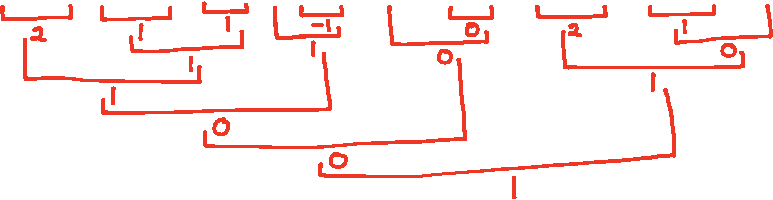
\includegraphics[width=6.07in]{\docImageDir/operators}
    }
    \vfill

\end{itemize}

% }}}
% -----------------------------------------------------------------------------
%   \standard{control flow}
% {{{

\newpage

\section{Question}
\standards{
  \standard{control flow}
}

Use two \mintinline{cpp}{for} loops (one inside the other, and without any
conditionals) to obtain the following output:

\inputminted[label=Output]{cpp}{\docCodeDir/.control.gen.output}
\textAnswer{\inputminted{cpp}{\docCodeDir/.control.cpp.gen.section.all}}

% }}}
% -----------------------------------------------------------------------------
%   \standard{arrays}
% {{{

\newpage

\section{Question}
\standards{
  \standard{arrays}
}

% mostly from reassessment-02

\section*{Instructions}

For questions with a picture illustrating memory, assume that the memory slots
are one \mintinline{cpp}{int} wide, and use ``?'' in a slot to indicate that it
contains an undefined value.  For each array, label an appropriately sized
group of slots with the array name, and fill in the slots with the array's
values.

\vspace{2.7ex}
\begin{minipage}[t]{0.5\linewidth} \vspace{0ex}
  \vspace{-2.7ex}
  \memoryImage
  \par
  \vspace{-0.63in}
  \hspace{0.45in}
  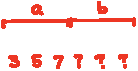
\includegraphics[width=1.15in]{\docImageDir/arrays-example}
\end{minipage}
\begin{minipage}[t]{0.5\linewidth} \vspace{0ex}
  \inputminted{cpp}{\docCodeDir/.arrays-example.cpp.gen.section.array}
\end{minipage}

\section*{Questions}

\begin{itemize}

  \item What is the index of the first element of an array?
    \textAnswer{\par
      Answer: \mintinline{cpp}{0}
    }
    \vfill

  \item What is the index of the last element of any array that holds 3 values?
    \textAnswer{\par
      Answer: \mintinline{cpp}{2}
    }
    \vfill

  \item What happens when you access an element of the array that does not
    exist?
    \textAnswer{\par
      If the program is allowed to access the location in memory then that
      location in memory is accessed as if it were an element of the array
      (regardless of what's actually there).  If the program doesn't have
      access to the location in memory, a segmentation fault (segfault) will
      occur, and the operating system will kill the process.
    }
    \vfill
    \vfill

  \item \memoryImage
    \textAnswer{\par
      \par
      \vspace{-1.12in}
      \hspace{0.9in}
      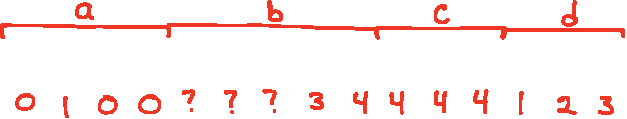
\includegraphics[width=5.2in]{\docImageDir/arrays}
    }
    \inputminted{cpp}{\docCodeDir/.arrays.cpp.gen.section.array}

\end{itemize}

% }}}
% -----------------------------------------------------------------------------
%   \standard{functions}
% {{{

\newpage

\section{Question}
\standards{
  \standard{functions}
}

% mostly from reassessment-03

Assuming that all necessary headers have been included and all required symbols
are in the standard namespace, do the following:

\begin{itemize}

  \item Write the prototype and definition for a function named
    \mintinline{cpp}{max} that accepts two \mintinline{cpp}{float}s and returns
    the largest as a \mintinline{cpp}{float}.
    \textAnswer{\inputminted{cpp}{\docCodeDir/.functions.cpp.gen.section.max}}
    \vfill

  \item Write the prototype and definition for a function named
    \mintinline{cpp}{change} that accepts two \mintinline{cpp}{int}s, both
    passed by reference, sets the value of each to twice its original value,
    and returns \mintinline{cpp}{void}.
    \textAnswer{\inputminted{cpp}{\docCodeDir/.functions.cpp.gen.section.set}}
    \vfill

  \item Write a short \mintinline{cpp}{main()} and \textbf{indicate its
    output}.  Your \mintinline{cpp}{main()} must begin with
    \mintinline{cpp}{int a = 2, b = 1;} and accomplish the following:
    \begin{itemize}
      \item Output the value of \mintinline{cpp}{max} called with the arguments
        \mintinline{cpp}{a} and \mintinline{cpp}{b}, followed by a newline.
      \item Call \mintinline{cpp}{change} with the arguments
        \mintinline{cpp}{a}  and \mintinline{cpp}{b}.
      \item Output the values of \mintinline{cpp}{a} and \mintinline{cpp}{b},
        separated by whitespace.
    \end{itemize}
    \textAnswer{\showCodeLeft{functions}{main}}
    \vfill

\end{itemize}

% }}}
% -----------------------------------------------------------------------------
%   \standard{file I/O}
% {{{

\newEvenPage

\section{Question}
\standards{
  \standard{file I/O}
}

% mostly from reassessment-04

Given

\inputminted[label={file-io-input.txt}]{text}{\docCodeDir/file-io-input.txt}

write an entire program (including \mintinline{cpp}{#include} directives and
\mintinline{cpp}{using} statements) to generate

\inputminted[label={file-io-output.gen.txt}]{text}{\docCodeDir/file-io-output.gen.txt}

without hard coding the number of integers to read in.  Be sure to check that
opening each file succeeded before reading from or writing to it, and
\mintinline{cpp}{return 1} from \mintinline{cpp}{main()} if it did not.

\newpage

\textQuestion{\makePageQuadrilleRuled}
\textAnswer{\inputminted{cpp}{\docCodeDir/file-io.cpp}}

% }}}
% -----------------------------------------------------------------------------
%   \standard{review :: general knowledge}
% {{{

\newpage

\section{Question}
\standards{
  \standard{review :: general knowledge}
}

Define or describe each of the following:
\textQuestion{\makeDashedLine}
\begin{itemize}
  \item C++ compilation process
    \begin{itemize}
      \item preprocess
        \textAnswer{\par
          \url{http://faculty.cs.niu.edu/~mcmahon/CS241/Notes/compile.html}
        }
        \vfill\textQuestion{\makeDashedLine}
      \item compile
        \textAnswer{\par
          \url{http://faculty.cs.niu.edu/~mcmahon/CS241/Notes/compile.html}
        }
        \vfill\textQuestion{\makeDashedLine}
      \item assemble
        \textAnswer{\par
          \url{http://faculty.cs.niu.edu/~mcmahon/CS241/Notes/compile.html}
        }
        \vfill\textQuestion{\makeDashedLine}
      \item link
        \textAnswer{\par
          \url{http://faculty.cs.niu.edu/~mcmahon/CS241/Notes/compile.html}
        }
        \vfill\textQuestion{\makeDashedLine}
    \end{itemize}
  \item program execution process
    \begin{itemize}
      \item load
        \textAnswer{\par
          \url{https://en.wikipedia.org/wiki/Loader_(computing)}
        }
        \vfill\textQuestion{\makeDashedLine}
      \item run
        \textAnswer{\par
          \url{https://en.wikipedia.org/wiki/Execution_(computing)}
        }
        \vfill\textQuestion{\makeDashedLine}
    \end{itemize}
  \item named constant vs object-like macro
    (e.g.~\mintinline{cpp}{const int ten = 10;} vs
    \mintinline{cpp}{#define TEN 10})
    \textAnswer{\par
      A named constant is like a variable except that its value cannot be
      changed, while an object-like macro is (roughly) a string of code that
      will be replaced by the preprocessor with some other string of code
      before compilation.  This has many implications, depending on how each is
      used, though in many simple cases (with compiler optimization on) the
      generated code is the same.
      \begin{itemize}
        \item \url{http://duramecho.com/ComputerInformation/WhyHowCppConst.html}
        \item \url{https://gcc.gnu.org/onlinedocs/cpp/Object-like-Macros.html}
      \end{itemize}
    }
    \vfill\textQuestion{\makeDashedLine}
  \item bit, byte, word
    \textAnswer{\par
      \begin{itemize}
        \item \url{https://en.wikipedia.org/wiki/Bit}
        \item \url{https://en.wikipedia.org/wiki/Byte}
        \item \url{https://en.wikipedia.org/wiki/Word_(computer_architecture)}
      \end{itemize}
    }
    \vfill
\end{itemize}

% }}}
% -----------------------------------------------------------------------------
%   \standard{object-oriented programming :: general knowledge}
% {{{

\newpage

\section{Question}
\standards{
  \standard{object-oriented programming :: general knowledge}
}

% from quiz-09

Give brief definitions of the following terms:
\textQuestion{\makeDashedLine}
\begin{itemize}
  \item object
    \textAnswer{\par
      A collection of data (what the object is made of) and methods (or member
      functions) on that data (what the object can do, or what messages the
      object understands) having a type (what the object is seen as).
    }
    \vfill\vfill\textQuestion{\makeDashedLine}
  \item class
    \textAnswer{\par
      A description of (or a template (though not in the C++ and Java sense) for
      creating) an object.
    }
    \vfill\textQuestion{\makeDashedLine}
  \item instance
    \textAnswer{\par
      A specific object existing in memory.
    }
    \vfill\textQuestion{\makeDashedLine}
  \item superclass
    \textAnswer{\par
      A class that is a parent of the class to which we are referring (i.e.~a
      class from which we directly or indirectly inherit).
    }
    \vfill\textQuestion{\makeDashedLine}
  \item subclass
    \textAnswer{\par
      A class that is a child of the class to which we are referring (i.e.~a
      class that directly or indirectly inherits from us).
    }
    \vfill\textQuestion{\makeDashedLine}
  \item member
    \textAnswer{\par
      A datum or method belonging to a class.
    }
    \vfill\textQuestion{\makeDashedLine}
  \item method
    \textAnswer{\par
      Or member function.  An action that an object is able to perform, or a
      message that an object is able to understand.
    }
    \vfill\textQuestion{\makeDashedLine}
  \item getters and setters
    \textAnswer{\par
      Methods used for retrieving (getting) or modifying (setting) an object's
      data members.
    }
    \vfill\textQuestion{\makeDashedLine}
  \item accessors and mutators
    \textAnswer{\par
      The same as getters and setters.
    }
    \vfill\textQuestion{\makeDashedLine}
  \item access modifiers
    \begin{itemize}
      \item public
        \textAnswer{\par
          Visible to everyone.
        }
        \vfill\textQuestion{\makeDashedLine}
      \item private
        \textAnswer{\par
          Visible within the class, and to friends.
        }
        \vfill\textQuestion{\makeDashedLine}
      \item protected
        \textAnswer{\par
          Visible within the class, to child classes, and to friends.
        }
        \vfill
    \end{itemize}
\end{itemize}

% }}}
% -----------------------------------------------------------------------------

\end{document}

